% defer/refcnt.tex

\section{Reference Counting}
\label{sec:defer:Reference Counting}

{ \scriptsize
\begin{verbbox}
 1 struct route_entry {
 2   atomic_t re_refcnt;
 3   struct route_entry *re_next;
 4   unsigned long addr;
 5   unsigned long iface;
 6   int re_freed;
 7 };
 8 struct route_entry route_list;
 9 DEFINE_SPINLOCK(routelock);
10
11 static void re_free(struct route_entry *rep)
12 {
13   ACCESS_ONCE(rep->re_freed) = 1;
14   free(rep);
15 }
16
17 unsigned long route_lookup(unsigned long addr)
18 {
19   int old;
20   int new;
21   struct route_entry *rep;
22   struct route_entry **repp;
23   unsigned long ret;
24
25 retry:
26   repp = &route_list.re_next;
27   rep = NULL;
28   do {
29     if (rep &&
30         atomic_dec_and_test(&rep->re_refcnt))
31       re_free(rep);
32     rep = ACCESS_ONCE(*repp);
33     if (rep == NULL)
34       return ULONG_MAX;
35     do {
36       if (ACCESS_ONCE(rep->re_freed))
37         abort();
38       old = atomic_read(&rep->re_refcnt);
39       if (old <= 0)
40         goto retry;
41       new = old + 1;
42     } while (atomic_cmpxchg(&rep->re_refcnt,
43                             old, new) != old);
44     repp = &rep->re_next;
45   } while (rep->addr != addr);
46   ret = rep->iface;
47   if (atomic_dec_and_test(&rep->re_refcnt))
48     re_free(rep);
49   return ret;
50 }
\end{verbbox}
}
\begin{figure}[bp]
\centering
\theverbbox
\caption{Reference-Counted Pre-BSD Routing Table Lookup}
\label{fig:defer:Reference-Counted Pre-BSD Routing Table Lookup}
\end{figure}

{ \scriptsize
\begin{verbbox}
 1 int route_add(unsigned long addr,
 2               unsigned long interface)
 3 {
 4   struct route_entry *rep;
 5
 6   rep = malloc(sizeof(*rep));
 7   if (!rep)
 8     return -ENOMEM;
 9   atomic_set(&rep->re_refcnt, 1);
10   rep->addr = addr;
11   rep->iface = interface;
12   spin_lock(&routelock);
13   rep->re_next = route_list.re_next;
14   rep->re_freed = 0;
15   route_list.re_next = rep;
16   spin_unlock(&routelock);
17   return 0;
18 }
19
20 int route_del(unsigned long addr)
21 {
22   struct route_entry *rep;
23   struct route_entry **repp;
24
25   spin_lock(&routelock);
26   repp = &route_list.re_next;
27   for (;;) {
28     rep = *repp;
29     if (rep == NULL)
30       break;
31     if (rep->addr == addr) {
32       *repp = rep->re_next;
33       spin_unlock(&routelock);
34       if (atomic_dec_and_test(&rep->re_refcnt))
35         re_free(rep);
36       return 0;
37     }
38     repp = &rep->re_next;
39   }
40   spin_unlock(&routelock);
41   return -ENOENT;
42 }
\end{verbbox}
}
\begin{figure}[bp]
\centering
\theverbbox
\caption{Reference-Counted Pre-BSD Routing Table Add/Delete}
\label{fig:defer:Reference-Counted Pre-BSD Routing Table Add/Delete}
\end{figure}

Reference counting tracks the number of references to a given object in
order to prevent that object from being prematurely freed.
As such, it has a long an honorable history of use dating back to
at least the early
1960s~\cite{Weizenbaum:1963:SLP:367593.367617}.\footnote{
	Weizenbaum discusses reference counting as if it was already
	well-known, so it likely dates back to the 1950s and perhaps
	even to the 1940s.
	And perhaps even further.
	People repairing and maintaining large machines have long
	used a mechanical reference-counting technique, where each
	worker had a padlock.}
Reference counting is thus an excellent candidate for a concurrent
implementation of Pre-BSD routing

To that end,
Figure~\ref{fig:defer:Reference-Counted Pre-BSD Routing Table Lookup}
shows data structures and the \co{route_lookup()} function and
Figure~\ref{fig:defer:Reference-Counted Pre-BSD Routing Table Add/Delete}
shows the \co{route_add()} and \co{route_del()} functions
(all at \path{route_refcnt.c}).
Since these algorithms are quite similar to the sequential algorithm
shown in
Figure~\ref{fig:defer:Sequential Pre-BSD Routing Table},
only the differences will be discussed.

Starting with
Figure~\ref{fig:defer:Reference-Counted Pre-BSD Routing Table Lookup},
line~2 adds the actual reference counter, line~6 adds a \co{->re_freed}
use-after-free check field, line~9 adds the \co{routelock} that will
be used to synchronize concurrent updates,
and lines~11-15 add \co{re_free()}, which sets
\co{->re_freed}, enabling \co{route_lookup()} to check for
use-after-free bugs.
In \co{route_lookup()} itself, lines~29-31 release the reference
count of the prior element and free it if the count becomes zero,
and lines~35-43 acquire a reference on the new element, with lines~36
and~37 performing the use-after-free check.

\QuickQuiz{}
	Why bother with a use-after-free check?
\QuickQuizAnswer{
	To greatly increase the probability of finding bugs.
	A small torture-test program
	(\path{routetorture.h}) that allocates and frees only
	one type of structure can tolerate a surprisingly
	large amount of use-after-free misbehavior.
	See Figure~\ref{fig:debugging:Number of Tests Required for 99 Percent Confidence Given Failure Rate}
	on page~\pageref{fig:debugging:Number of Tests Required for 99 Percent Confidence Given Failure Rate}
	and the related discussion in
	Section~\ref{sec:debugging:Hunting Heisenbugs}
	starting on
	page~\pageref{sec:debugging:Hunting Heisenbugs}
	for more on the importance
	of increasing the probability of finding bugs.
} \QuickQuizEnd

In Figure~\ref{fig:defer:Reference-Counted Pre-BSD Routing Table Add/Delete},
lines~12, 16, 25, 33, and~40 introduce locking to synchronize
concurrent updates.
Line~14 initializes the \co{->re_freed} use-after-free-check field,
and finally lines~34-35 invoke \co{re_free()} if the new value of
the reference count is zero.

\QuickQuiz{}
	Why doesn't \co{route_del()} in
	Figure~\ref{fig:defer:Reference-Counted Pre-BSD Routing Table Add/Delete}
	use reference counts to
	protect the traversal to the element to be freed?
\QuickQuizAnswer{
	Because the traversal is already protected by the lock, so
	no additional protection is required.
} \QuickQuizEnd

\begin{figure}[tb]
\centering
\resizebox{2.5in}{!}{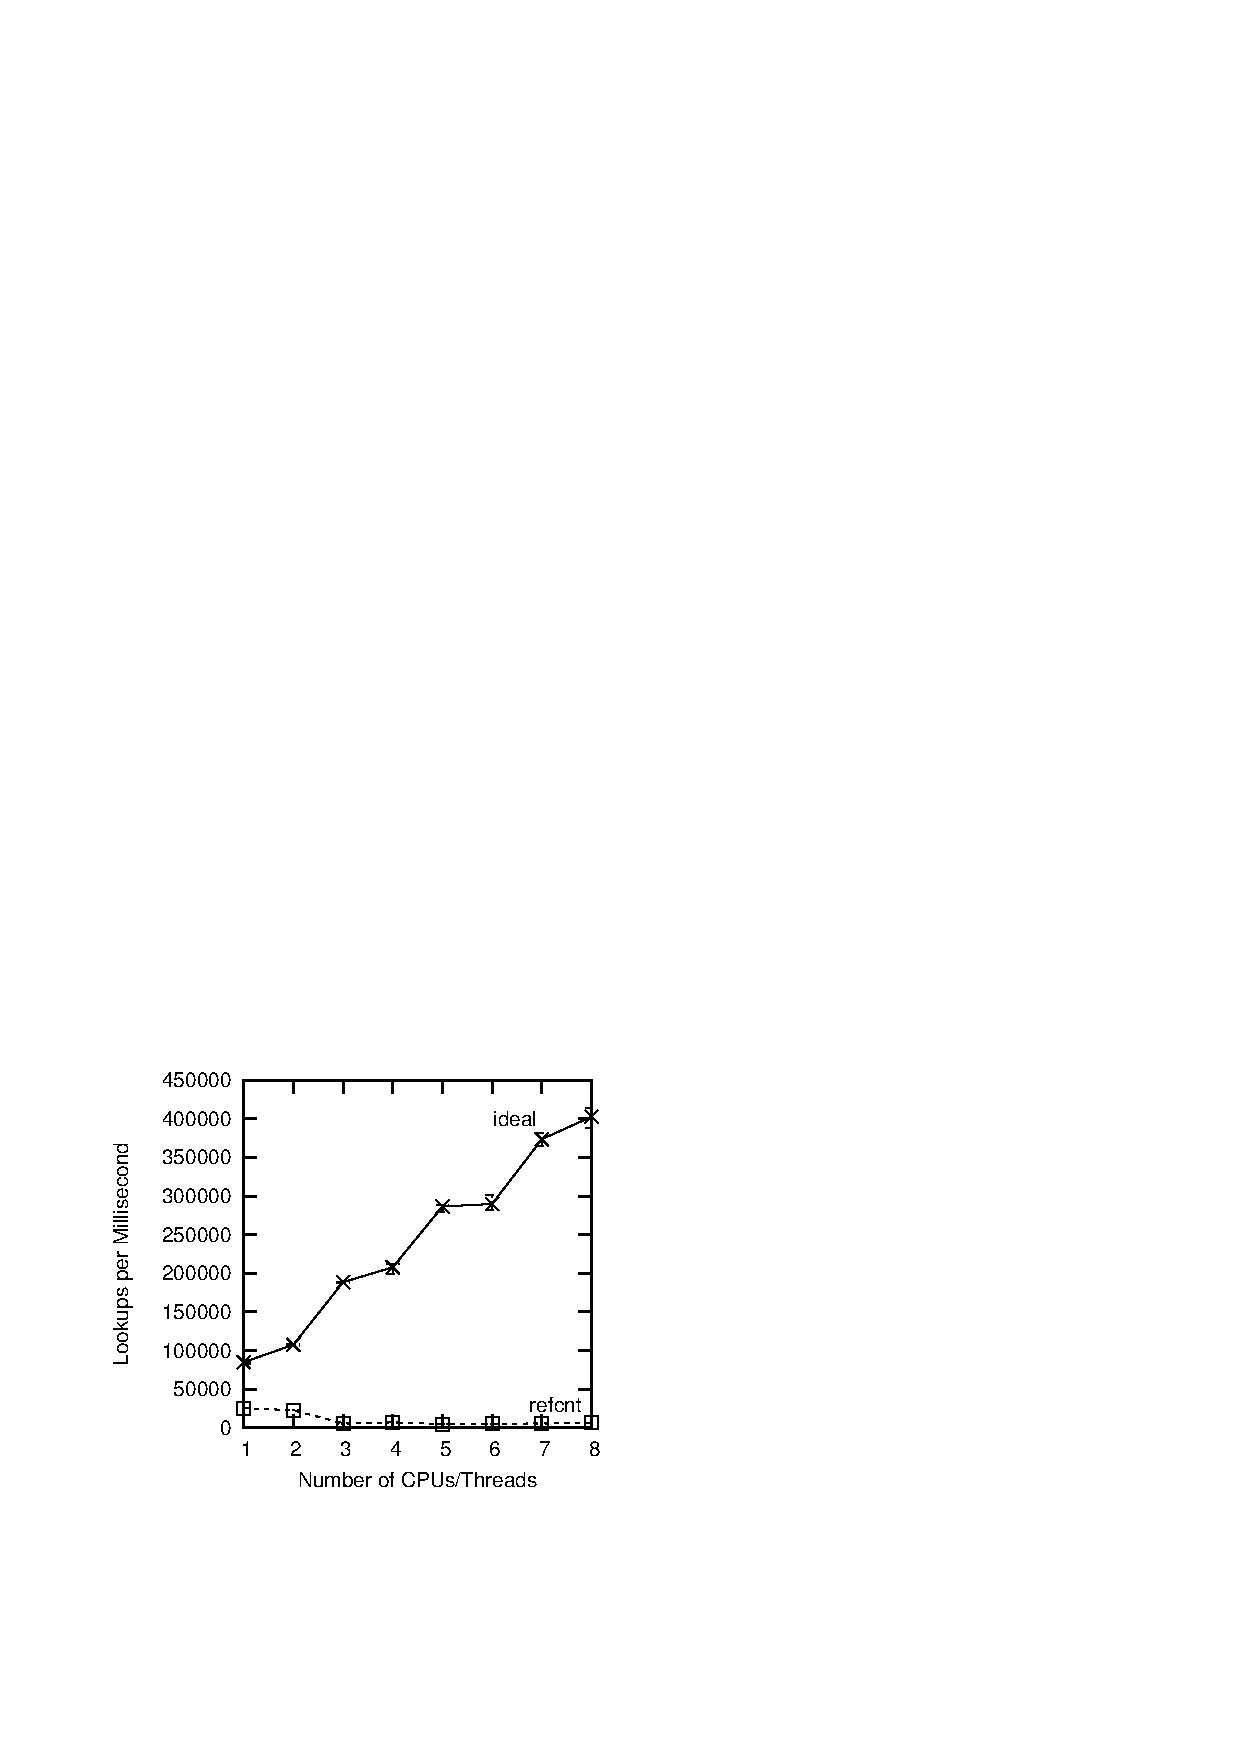
\includegraphics{CodeSamples/defer/data/paulmck.2016/perf-refcnt}}
\caption{Pre-BSD Routing Table Protected by Reference Counting}
\label{fig:defer:Pre-BSD Routing Table Protected by Reference Counting}
\end{figure}

Figure~\ref{fig:defer:Pre-BSD Routing Table Protected by Reference Counting}
shows the performance and scalability of reference counting on a
read-only workload with a ten-element list running on a
single-socket four-core hyperthreaded 2.5GHz x86 system.
The ``ideal'' trace was generated by running the sequential code shown in
Figure~\ref{fig:defer:Sequential Pre-BSD Routing Table}.
The reference-counting performance is abysmal and its scalability even
more so, with the ``refcnt'' trace dropping down onto the x~axis.
This should be no surprise in view of
Chapter~\ref{chp:Hardware and its Habits}:
The reference-count acquisitions and releases have added frequent
shared-memory writes to an otherwise read-only workload, thus
incurring severe retribution from the laws of physics.
As well it should, given that all the wishful thinking in the world
is not going to increase the speed of light or decrease the size of
the atoms used in modern digital electronics.

\QuickQuiz{}
	Why the stairsteps in the ``ideal'' line in
	Figure~\ref{fig:defer:Pre-BSD Routing Table Protected by Reference Counting}?
	Shouldn't it be a straight line?
\QuickQuizAnswer{
	The stair-steps are due to hyperthreading.
	On this particular system, the hardware threads in a given
	core have consecutive CPU numbers.
	In addition, this particular pointer-following
	low-cache-miss-rate workload seems
	to allow a single hardware thread to consume most of the
	relevant resources within its core.
	Workloads featuring heavier computational loads should be
	expected to gain greater benefit from each core's second
	hardware thread.
} \QuickQuizEnd

But it gets worse.

Running multiple updater threads repeatedly invoking
\co{route_add()} and \co{route_del()} will quickly encounter the
\co{abort()} statement on line~37 of
Figure~\ref{fig:defer:Reference-Counted Pre-BSD Routing Table Lookup},
which indicates a use-after-free bug.
This in turn means that the reference counts are not only profoundly
degrading scalability and performance, but also failing to provide
the needed protection.

One sequence of events leading to the use-after-free bug is as follows,
given the list shown in
Figure~\ref{fig:defer:Pre-BSD Packet Routing List}:

\begin{enumerate}
\item	Thread~A looks up address~42, reaching line~33 of
	\co{route_lookup()} in
	Figure~\ref{fig:defer:Reference-Counted Pre-BSD Routing Table Lookup}.
	In other words, Thread~A has a pointer to the first element,
	but has not yet acquired a reference to it.
\item	Thread~B invokes \co{route_del()} in
	Figure~\ref{fig:defer:Reference-Counted Pre-BSD Routing Table Add/Delete}
	to delete the route entry for address~42.
	It completes successfully, and because this entry's \co{->re_refcnt}
	field was equal to the value one, it invokes
	\co{re_free()} to set the \co{->re_freed} field and to free the entry.
\item	Thread~A continues execution of \co{route_lookup()}.
	Its \co{rep} pointer is non-\co{NULL}, but line~36 sees that
	its \co{->re_freed} field is non-zero, so line~37 invokes
	\co{abort()}.
\end{enumerate}

The problem is that the reference count is located in the object
to be protected, but that means that there is no protection during
the instant in time when the reference count itself if being acquired!
This is the reference-counting counterpart of a locking issue noted
by Gamsa et al.~\cite{Gamsa99}.
One could imagine using a global lock or reference count to protect
the per-route-entry reference-count acquisition, but this would
result in severe contention issues.
Although algorithms exist that allow safe reference-count acquisition
in a concurrent environment~\cite{Valois95a}, they are not only extremely
complex and error-prone~\cite{MagedMichael95a}, but also provide
terrible performance and scalability~\cite{ThomasEHart2007a}.

In short, concurrency has most definitely reduced the usefulness
of reference counting!

\QuickQuiz{}
	If concurrency has ``most definitely reduced the usefulness
	of reference counting'', why are there so many reference
	counters in the Linux kernel?
\QuickQuizAnswer{
	That sentence did say ``reduced the usefulness'', not
	``eliminated the usefulness'', now didn't it?

	Please see
	Section~\ref{sec:together:Refurbish Reference Counting},
	which discusses some of the techniques that the Linux kernel
	uses to take advantage of reference counting in a highly
	concurrent environment.
} \QuickQuizEnd

That said, sometimes it is necessary to look at a problem in an
entirely different way in order to successfully solve it.
The next section describes what could be thought of as an
inside-out reference count that provides decent performance
and scalability.
